\documentclass{report}
\usepackage{nth}
\usepackage{fancyhdr}
\pagestyle{fancy}
\usepackage{titlesec}
\usepackage{amsmath}
\usepackage{amssymb}
\usepackage{graphicx}
\usepackage{csquotes}
\usepackage{hyperref}


\fancyhead[L]{Interazione Uomo Macchina}
\fancyhead[R]{Marco Ferrara}

\setlength{\headheight}{15pt}

\title{IUM - Interazione Uomo Macchina}
\author{Marco Ferrara}
\date{Ottobre 2024}

\begin{document}
	\maketitle
	\tableofcontents
	\newpage
	
	\chapter{Introduzione}
	L'obiettivo del corso è quello di fornire un primo orientamento sulle problematiche del \textbf{design} e della \textbf{valutazione} dell'\textbf{interazione uomo-macchina}, per la progettazione di sistemi interattivi \textbf{facili da usare}, discutendo le qualità del software di interesse degli \textbf{utenti finali}.

	\section{Interfaccia Utente}
	La \textbf{interfaccia utente} è il mezzo attraverso il quale l'utente interagisce con un sistema o prodotto per raggiungere obiettivi specifici. Essa funge da punto di contatto tra l'utente e il sistema, rendendo possibile la comunicazione e la gestione delle funzionalità offerte. Un'interfaccia utente efficace non solo facilita l'uso del sistema, ma si adatta ai bisogni e alle aspettative dell'utente, risultando essenziale per un'esperienza utente intuitiva e soddisfacente.

	\section{HCI – Human-Computer Interaction}
	E' la disciplina che si occupa della progettazione, valutazione e realizzazione di sistemi interattivi basati su computer destinati all'uso umano e dello studio dei principali fenomeni che li circondano.
	\vspace{\baselineskip} \\
	Ha le sue origini in due aree disciplinari molto diverse:
	\begin{itemize}
		\item \textbf{Ergonomia}: si occupa dei problemi relativi al lavoro umano in rapporto alla progettazione delle macchine e degli ambienti di lavoro, cercando di ottimizzare il comfort, la sicurezza e l'efficienza dell'utente.

		\item \textbf{Scienza dei Computer}: si occupa della progettazione e realizzazione di sistemi software, includendo sia aspetti teorici che pratici come l'architettura dei sistemi e la programmazione.
	\end{itemize}

	I principali temi su cui si basa l'HCI sono:

	\begin{itemize}
		\item Metodologie e processi per la \textbf{progettazione} delle interfacce fra uomo e computer: studio e definizione delle migliori pratiche per creare interfacce intuitive e accessibili.

		\item Metodi e strumenti per la \textbf{realizzazione} delle interfacce: utilizzo di tecniche di sviluppo e software specifici per implementare le interfacce progettate.

		\item Tecniche per la \textbf{valutazione} e il confronto delle interfacce: approcci empirici e analitici per misurare l'efficacia e l'efficienza delle interfacce in contesti reali o simulati.

		\item Progettazione di nuove \textbf{tecniche di interazione}: esplorazione di modalità innovative per interagire con i sistemi, come interfacce vocali, touch, o realtà aumentata.

		\item Sviluppo di \textbf{teorie} e \textbf{modelli} descrittivi e predittivi dell'interazione uomo-computer: costruzione di modelli teorici per comprendere e prevedere i comportamenti degli utenti durante l'interazione con i sistemi.

		\item \ldots
	\end{itemize}
	L'Human-Computer Interaction (HCI) è una disciplina che nasce dall'integrazione di diverse aree del sapere, ognuna delle quali contribuisce alla sua complessità e alla sua applicazione pratica. In particolare, l'HCI trae ispirazione e strumenti da tre principali campi disciplinari: la \textbf{Scienza dei computer}, la \textbf{Scienza della progettazione} e le \textbf{Scienze dell'uomo}:

	\begin{itemize}
    	\item \textbf{Scienza dei computer}: In quest'area si trovano i paradigmi di interazione, che definiscono il modo in cui gli utenti interagiscono con i dispositivi digitali. Comprende anche lo sviluppo di device di interazione e la programmazione delle interfacce utente (UI programming). Inoltre, si studiano i modelli di dialogo tra uomo e macchina, la computer graphics e le tecniche di visualizzazione delle informazioni, oltre all'intelligenza artificiale, che offre nuove possibilità di interazione e automazione. 
    	
    	\item \textbf{Scienza della progettazione}: Qui rientrano l'interaction design e l'industrial design, che si concentrano sulla progettazione ergonomica e funzionale di sistemi e interfacce. Si studiano anche l'architettura dell'informazione, le tecniche di valutazione dell'usabilità e dell'esperienza utente, e il project management, che garantisce la corretta gestione dei progetti legati alla progettazione di interfacce.
    	
    	\item \textbf{Scienze dell'uomo}: Questa area include la psicologia, le scienze cognitive, la psicologia sociale, la linguistica e le scienze della comunicazione. Queste discipline studiano il comportamento umano, i processi mentali, le dinamiche sociali e linguistiche, e come queste influenzano l'interazione con i sistemi informatici. 
	\end{itemize}
	L'HCI si posiziona dunque al centro di queste tre grandi aree, con l'obiettivo di creare interfacce utente che siano non solo funzionali e tecnologicamente avanzate, ma anche ottimizzate per l'uso umano, tenendo conto dei bisogni cognitivi, fisici e sociali dell'utente. Così facendo va a fondere due discipline complicate con background culturali molto diversi: la psicologia e la programmazione.

	\chapter{Accettabilità di un sistema software}
	L'accessibilità di un sistema software è la capacità di essere utilizzato da quante più persone possibili, indipendentemente dalle loro capacità fisiche, cognitive o sensoriali. 

	La sua definizione si è evoluta nel tempo vedendo due principali accezioni riconosiute ufficialmente dalla comunità scientifica.

	\section{Definizione di Jacob Nielsen - 1993}
	L'accettabilità di un sistema software, secondo Jacob Nielsen, è la misura in cui un software viene considerato idoneo all'uso dagli utenti finali. Tale accettabilità è influenzata da diversi fattori, che possono essere suddivisi in due categorie principali: le caratteristiche generali del sistema e le proprietà legate all'usabilità.
	\begin{itemize}
		\item \textbf{Costo}: che deve essere commisurato alle risorse disponibili e al valore percepito del software.
		\item \textbf{Compatibilità}: con altri sistemi e dispositivi con cui si interfaccia, facilitando la sua integrazione nell'ambiente lavorativo o personale.
		\item \textbf{Affidabilità}: Il sistema deve essere stabile e funzionare senza problemi, garantendo un basso tasso di malfunzionamenti o errori.
		\item \textbf{Utilità}: Rappresenta la capacità del software di soddisfare i bisogni pratici dell'utente, fornendo le funzionalità necessarie per raggiungere gli obiettivi prefissati.
		\item \textbf{Utilizzabilità}: Questa componente riguarda il grado di facilità con cui gli utenti possono utilizzare il sistema. Si divide a sua volta in diversi fattori chiave legati all'usabilità.
	\end{itemize}
	L'usabilità si compone di più fattori:
	\begin{itemize}
		\item \textbf{Facilità di apprendimento}: Indica quanto rapidamente un nuovo utente può apprendere l'uso del software, riducendo il tempo necessario per diventare operativo.
		\item \textbf{Facilità d'uso}: Si riferisce alla semplicità di interazione quotidiana con il sistema, che non dovrebbe richiedere sforzi occessivi per compiere operazioni comuni.
		\item \textbf{Facilità di memorizzazione}: Riguarda la capacità dell'utente di ricordare facilmente come utilizzare il sistema anche dopo lunghi periodi di inattività.
		\item \textbf{Numero ridotto di errori commessi dall'utente}: Un sistema ben progettato dovrebbe minimizzare la possibilità che l'utente commetta errori e, in caso di errore, offrire una facile via di recupero.
		\item \textbf{Soddisfazione nell'uso}: L'utente deve provare una sensazione positiva nell'uso del sistema, che dovrebbe risultare piacevole e gratificante.
	\end{itemize}

	\section{Definizione di ISO 9241-11 - 1998}
	La nuova versione elabora i concetti di versioni precedenti e li espande, introducendo nuovi concetti e definizioni. In particolare, l'ISO 9241-11 definisce l'usabilità come
	\begin{center}
	\enquote{
		la misura in cui un \textbf{sistema}, prodotto o \textbf{servizio} può essere utilizzato da utenti \textit{specifici} per raggiungere obiettivi \textit{specifici} con efficacia, efficienza e soddisfazione in uno \textit{specifico} contesto d'uso.
	}
	\end{center}
	L'usabilità, in questo caso, non è più un concetto assoluto ma relativo, che dipende da vari fattori come gli utenti, gli obiettivi e il contesto d'uso.\\
	Questa definizione introduce tre nuovi concetti chiave:
	\begin{itemize}
		\item \textbf{Efficacia}: Indica la capacità del sistema di consentire all'utente di raggiungere i propri obiettivi in modo accurato e completo senza conseguenze negative.
		\item \textbf{Efficienza}: Si riferisce alla capacità del sistema di consentire all'utente di raggiungere i propri obiettivi con un impiego minimo di risorse, come tempo, sforzo e costi.
		\item \textbf{Soddisfazione}: Rappresenta il grado di piacere e gratificazione che l'utente prova nell'utilizzare il sistema, derivante da una combinazione di fattori come l'usabilità, l'estetica e l'esperienza d'uso (UX).
	\end{itemize}

	\section{Confronto tra le due definizioni}
	Le due definizioni di accettabilità hanno diverse caratteristiche, ma sono anche diverse in conseguenza. La prima definizione è basata su una visione più generale e pratica dell'accettabilità, che include aspetti come costo, compatibilità e affidabilità, oltre alle proprietà legate all'usabilità. La seconda definizione, invece, è più specifica e focalizzata sull'usabilità, definendo l'accettabilità come la capacità di un sistema di consentire agli utenti di raggiungere i propri obiettivi in modo efficace, efficiente e soddisfacente.\\
	Il confronto tra le due definizioni può essere facilmente illustrata con un esempio. Supponiamo di considerare due sistemi software, A e B, che hanno le seguenti caratteristiche:
	\begin{itemize}
		\item Sistema A: è molto costoso ma altamente affidabile e compatibile con altri sistemi. Tuttavia, è difficile da imparare e usare, e gli utenti commettono frequentemente errori nell'interazione con il sistema.
		\item Sistema B: è economico, facile da imparare e usare, e gli utenti sono soddisfatti dell'esperienza d'uso. Tuttavia, è meno affidabile e compatibile rispetto al sistema A.
	\end{itemize}
	Secondo la definizione di Jacob Nielsen, il sistema A potrebbe essere considerato più accettabile rispetto al sistema B, poiché ha caratteristiche come costo, affidabilità e compatibilità che lo rendono idoneo all'uso. Tuttavia, secondo la definizione ISO 9241-11, il sistema B potrebbe essere considerato più accettabile, poiché consente agli utenti di raggiungere i propri obiettivi in modo efficace, efficiente e soddisfacente, nonostante le sue limitazioni in termini di affidabilità e compatibilità.\\
	In conclusione, entrambe le definizioni forniscono un quadro utile per valutare l'accettabilità di un sistema software, ma si concentrano su aspetti diversi e possono portare a conclusioni diverse a seconda del contesto e degli obiettivi specifici dell'utente.

	\section{User eXperience (UX) nell'ISO 9241-210}
	L'ISO 9241-210 definisce l'esperienza utente (UX) come \enquote{le percezioni e le reazioni di un utente che derivano dall'uso o dall'aspettativa d'uso di un prodotto, sistema o servizio}. Questa definizione sottolinea l'importanza di considerare non solo l'usabilità di un sistema, ma anche l'esperienza complessiva dell'utente durante l'interazione con esso. L'esperienza utente include le emozioni dell'utente, le sue preferenze, le reazioni psicologiche e fisiche e i comportamenti che si verificano prima, durante e dopo l'uso del sistema.

	\section{Obiettivi dell'usabilità}
	L'usabilità è un concetto multidimensionale che può essere valutato attraverso diversi obiettivi, tra cui:
	\begin{itemize}
		\item \textbf{Efficacia}: Misura la capacità del sistema di consentire all'utente di raggiungere i propri obiettivi in modo accurato e completo senza conseguenze negative.
		\item \textbf{Efficienza}: Si riferisce alla capacità del sistema di consentire all'utente di raggiungere i propri obiettivi con un impiego minimo di risorse, come tempo, sforzo e costi.
		\item \textbf{Sicurezza nell'uso}: Indica la capacità del sistema di proteggere l'utente da situazioni di rischio o pericolo durante l'interazione, evitando errori o danni accidentali.
		\item \textbf{Soddisfazione}: Rappresenta il grado di piacere e gratificazione che l'utente prova nell'utilizzare il sistema, derivante da una combinazione di fattori come l'usabilità, l'estetica e l'esperienza d'uso (UX).
		\item \textbf{Facilità di apprendimento}: Indica quanto rapidamente un nuovo utente può apprendere l'uso del software, riducendo il tempo necessario per diventare operativo.
		\item \textbf{Facilità d'uso}: Si riferisce alla semplicità di interazione quotidiana con il sistema, che non dovrebbe richiedere sforzi occessivi per compiere operazioni comuni.
		\item \textbf{Facilità di memorizzazione}: Riguarda la capacità dell'utente di ricordare facilmente come utilizzare il sistema anche dopo lunghi periodi di inattività.
		\item \textbf{Presenza di features}: Indica la presenza di funzionalità e caratteristiche che facilitano l'uso del sistema e migliorano l'esperienza dell'utente.
	\end{itemize}
	Sicuramente, la UX non deve portare l'utente a provare sentimenti negativi come noia, frustrazione, sensi di colpa, confusione e così via. Altresì, l'utente deve provare sentimenti positivi come divertimento, soddisfazione, orgoglio, eccitazione, ecc.
	
	\section{Dalla Usability alla User eXperience}
	La User eXperience (UX) è un concetto più ampio e complesso rispetto all'usabilità, poiché include non solo la facilità d'uso di un sistema, ma anche le emozioni, le preferenze e le reazioni dell'utente durante l'interazione con esso. L'usabilità è un aspetto fondamentale della UX, ma non è l'unico fattore che contribuisce alla qualità complessiva dell'esperienza utente.
	\vspace{\baselineskip} \\
	Se l'efficienza mira a ridurre il tempo e lo sforzo necessari per raggiungere un obiettivo, in maniera semplice e senza errori, la UX coinvolge i sentimenti, i quali possono essere influenzati da attributi funzionali del sistema, come la portabilità o la robustezza, ma anche da attributi non funzionali, come l'usabilità e la privacy, fino ad arrivare a fattori specifici come il piacere nell'utilizzare il sistema, la motivazione o l'estetica.
	\vspace{\baselineskip} \\
	Un prodotto capace di generare una buona UX è in grado di soddisfare le esigenze e le aspettative dell'utente e dovrebbe essere utile, usabile e desiderabile. Per realizzare prodotti di successo, la UX enfatizza sul piacere dell'utente, sull'aestetica e sul divertimento. C'è una correlazione tra l'aestetica e la percezione della qualità dell'interfaccia. Interfacce appetibili dal punto di vista estetico sono percepite come più utili anche se lo sono meno rispetto a interfacce con funzionalità simili ma meno attraenti.
	
	\section{Migliorare l'interfaccia utente}
	Migliorare l'interfaccia utente di un sistema software è un processo continuativo che ha come scopo quello di rendere il sistema più facile da usare, più efficace e più soddisfacente per l'utente. Se pensiamo a questo processo in ambito business, possiamo dire che un'interfaccia ben progettata può portare a una maggiore produttività, a una riduzione degli errori e dei costi, a un aumento della soddisfazione dell'utente e, di conseguenza, a una maggiore competitività sul mercato.
	\vspace{\baselineskip} \\
	Di conseguenza, la progettazione e la valutazione dell'interfaccia utente dovrebbero essere parte integrante del processo di sviluppo del software, dall'inizio alla fine, coinvolgendo gli utenti fin dall'inizio per garantire che le loro esigenze e aspettative siano soddisfatte. L'usabilità e la user experience dovrebbero essere valutate in modo continuativo durante tutto il ciclo di vita del prodotto per identificare e risolvere i problemi di usabilità e migliorare l'esperienza dell'utente.
	\vspace{\baselineskip} \\
	Basarsi su linee guida e best practice di design, condurre test di usabilità e coinvolgere gli utenti nel processo di progettazione sono solo alcune delle strategie che possono essere adottate per migliorare l'interfaccia utente di un sistema software. 

	\section{Come ottenere l'usabilità}
	Per ottenere un'interfaccia utente usabile e una user experience soddisfacente, è necessario seguire alcune linee guida e best practice di design. Il punto di partenza è centrare il progetto sull'utente (User-Centred Design) andando a capire l'utente stesso, i suoi compiti e il contesto d'uso, sviluppando iterativamente prototipi e testandoli con gli utenti per valutare l'usabilità e l'esperienza d'uso. Inoltre, è importante adottare un approccio multidisciplinare, coinvolgendo esperti di diverse discipline come la psicologia, il design, l'informatica e l'ingegneria, per garantire che l'interfaccia utente sia progettata in modo efficace e soddisfacente per l'utente.
	\vspace{\baselineskip} \\
	Queste linee guida sono specificate in vari standard e raccomandazioni, come l'ISO 9241-210, che fornisce linee guida per la progettazione Human-Centred.

	\section{Human-Centred Design Prosess - ISO 9241-210}
	L'Human-Centred Design Process (HCD) è un approccio iterativo alla progettazione che mette l'utente al centro del processo, coinvolgendo gli utenti fin dall'inizio per garantire che le loro esigenze e aspettative siano soddisfatte.
	\begin{center}
		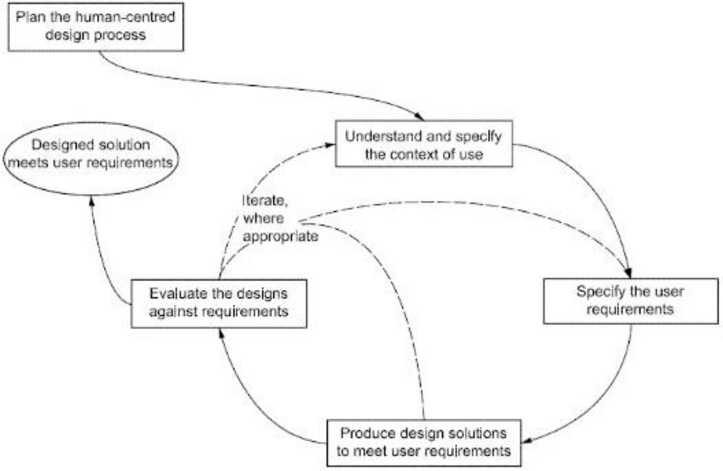
\includegraphics[scale=0.5]{assets/hcd.png}
	\end{center}
	Il processo HCD si divide in 6 fasi:
	\begin{enumerate}
		\item \textbf{Plan the human centred design process}: Definire gli obiettivi del progetto, identificare gli utenti e le loro esigenze, e pianificare le attività di progettazione e valutazione. Definendo il target di riferimento si possono identificare le caratteristiche necessarie per soddisfare le esigenze degli utenti, i metodi di coinvolgimento all'interno della progettaglione e di contatto con gli stessi e il metodo di raccolta delle informazioni da utilizzare.
		\item \textbf{Understand and specify the context of use}: Una volta definito il target e le caratteristiche, si procede con l'analisi del contesto d'uso, ovvero l'ambiente in cui il sistema verrà utilizzato, le attività che gli utenti dovranno svolgere e le caratteristiche degli utenti stessi. Questa fase è fondamentale per comprendere le esigenze e le aspettative degli utenti e per definire i requisiti del sistema.
		\item \textbf{Specify the user requirements}: Definire i requisiti funzionali e non dell'utente in base all'analisi del contesto d'uso, identificando le funzionalità e le caratteristiche che il sistema dovrà avere per soddisfare le esigenze degli utenti. Questi requisiti dovrebbero essere specifici, misurabili e verificabili, e dovrebbero essere utilizzati come base per la progettazione del sistema.
		\item \textbf{Produce design solutions to meet user requirements}: Sviluppare soluzioni di design che soddisfino i requisiti dell'utente, utilizzando tecniche di progettazione come la creazione di wireframes, mockup e prototipi. Queste soluzioni dovrebbero essere valutate con gli utenti per garantire che siano efficaci, efficienti e soddisfacenti. I prototipi non devono necessariamente essere completi, ma devono essere sufficientemente dettagliati per permettere agli utenti di valutare l'interfaccia, possono addirittura essere schizzi o storyboard.
		\item \textbf{Evaluate designs against requirements}: Valutare le soluzioni di design rispetto ai requisiti dell'utente, utilizzando tecniche di valutazione come i test di usabilità, le valutazioni euristiche e le analisi cognitive. Queste valutazioni dovrebbero essere condotte con gli utenti per identificare i problemi di usabilità e migliorare l'esperienza dell'utente. I test di usabilità possono essere condotti in laboratorio, in campo o in remoto, e possono coinvolgere diversi tipi di utenti, come utenti esperti o utenti novizi. Da questo punto, in base agli esiti delle valutazioni, si può tornare alla fase 2 per rivedere il contesto d'uso e ripetere il processo; oppure alla fase 3 per rivedere i requisiti utente e ripetere il processo; oppure alla fase 4 per rivedere le soluzioni di design e ripetere il processo; oppure avanzare alla fase 6.
		\item \textbf{Designed solutions meet user requirements}: Implementare le soluzioni di design finali che soddisfino i requisiti dell'utente, utilizzando tecniche di sviluppo come la programmazione e la progettazione dell'interfaccia utente. Queste soluzioni dovrebbero essere testate con gli utenti per garantire che siano efficaci, efficienti e soddisfacenti, e dovrebbero essere valutate in un contesto d'uso reale per verificare che soddisfino le esigenze degli utenti.
	\end{enumerate}

	\chapter{Requisiti, tecniche di raccolta dati e analisi dei task}
	\section{Requisiti di prodotto}
	I requisiti di prodotto sono le specifiche funzionali e non funzionali che definiscono le caratteristiche e le prestazioni del prodotto. Vengono raccolti in un documento strutturato che fornisce una descrizione dettagliata delle funzionalità, delle prestazioni e delle caratteristiche del prodotto, e che viene utilizzato come base per la progettazione e lo sviluppo del prodotto stesso. Essi vengono identificati attraverso analisi condotte con varie tecniche. 
	\vspace{\baselineskip}\\
	I requisiti di prodotto possono essere divisi in due categorie principali: requisiti funzionali e requisiti non funzionali. I requisiti funzionali definiscono le funzionalità che il sistema deve implementare per soddisfare le esigenze dell'utente, mentre i requisiti non funzionali definiscono le caratteristiche del sistema che non sono direttamente legate alle funzionalità, ma che influenzano la sua usabilità, la sua sicurezza e le sue prestazioni.
	\vspace{\baselineskip}\\
	I requisiti di prodotto possono essere definiti mediante diversi tipi di analisi:
	\begin{itemize}
		\item \textbf{Analisi dell'utente}: qual è il target di utenza del prodotto.
		\item \textbf{Analisi dei bisogni}: quali sono i bisogni e le esigenze degli utenti.
		\item \textbf{Analisi del contesto d'uso}: in quali contesti il prodotto verrà utilizzato.
		\item \textbf{Analisi degli scenari d'uso}: in quali modi diversi gli utenti interagiranno con il prodotto.
		\item \textbf{Analisi della concorrenza}: quali sono i prodotti simili presenti sul mercato. Quali sono i punti di forza e di debolezza rispetto ai prodotti concorrenti.
	\end{itemize}
	Si precisa che individuare e specificare i requisiti non significa progettare il prodotto, ma definire cosa il prodotto deve fare e come deve comportarsi. i requisiti pongono dei vincoli all'attività di progettazione. Il documento dei requisiti indica che cosa si deve realizzare e perchè, non come.
	\vspace{\baselineskip}\\
	La definizione dei requisiti può essere sintetizzata come nello schema che segue:
	\begin{center}
		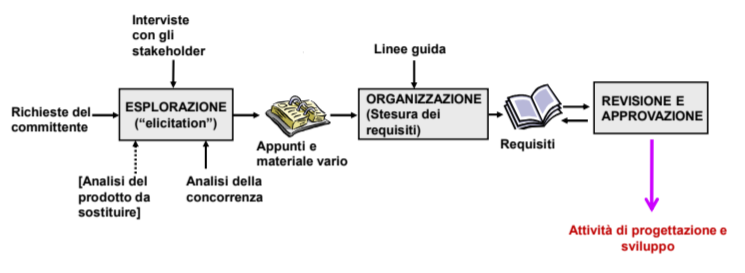
\includegraphics[scale=0.5]{assets/requisiti.png}
	\end{center}
	Si parte dalle richieste del committente, che includono le aspettative e le necessità per il prodotto o servizio da sviluppare. Da qui, si avvia la fase di esplorazione, durante la quale si conducono interviste con gli stakeholder, si analizzano prodotti simili già esistenti e si valuta la concorrenza. Tutte queste informazioni raccolte diventano appunti e materiali di riferimento.
	\vspace{\baselineskip}\\
	Successivamente, si passa alla organizzazione, dove questi dati vengono rielaborati per redigere un documento che descrive i requisiti necessari. Le linee guida servono come riferimento per questa stesura. Il risultato finale è un elenco di requisiti chiari e strutturati.
	\vspace{\baselineskip}\\
	Infine, questi requisiti vengono sottoposti a una fase di revisione e approvazione, dove si valuta se soddisfano le esigenze iniziali e, una volta approvati, si può procedere alle attività di progettazione e sviluppo.
	\vspace{\baselineskip}\\
	La raccolta dei requisiti è un'attività fondamentale e critica per il successo di un progetto. Durante questa fase, si possono presentare diversi problemi come:
	\begin{itemize}
		\item il rischio di ampliare/restringere essessivamente il campo di applicazione del progetto o i temi da approfondire;
		\item incomprensioni con gli utenti che spesso hanno una conoscenza limitata dei loro bisogni; o con chi raccoglie i requisiti che può non avere una conoscenza approfondita del dominio applicativo e può utilizzare un linguaggio differente da quello degli utenti;
		\item connflitto tra gli interessi dei vari stakeholder che possono avere esigenze contrastanti;
		\item volatilità dei requisiti, che possono cambiare nel tempo a causa di nuove esigenze o di nuove tecnologie.
	\end{itemize}
	Gli utenti sono coloro che decidono se utilizzare il prodotto, che hanno preferenze, abitudini e aspettative ogni qualvolta si vada ad utilizzare un prodotto. Non supportare le loro esigenze può provocare alti costi in termini di produttività per l'azienda e di frustrazione per l'utente a tal punto da mettere a rischio la riuscita del progetto.

	\section{Tecniche di raccolta dati}
	La raccolta dei dati è un'attività fondamentale per la definizione dei requisiti di un prodotto. Esistono diverse tecniche di raccolta dati che possono essere utilizzate per raccogliere informazioni sui bisogni e le esigenze degli utenti, sul contesto d'uso del prodotto e sulle funzionalità richieste. Alcune delle tecniche più comuni sono:
	\begin{itemize}
		\item \textbf{Interviste}: Conversazioni strutturate o semi-strutturate con gli utenti per raccogliere informazioni sui loro bisogni, aspettative e comportamenti.
		\item \textbf{Questionari}: Questionari strutturati per raccogliere informazioni quantitative sui bisogni e le preferenze degli utenti.
		\item \textbf{Osservazioni}: Osservazioni dirette degli utenti durante l'utilizzo del prodotto per identificare problemi di usabilità e migliorare l'esperienza dell'utente.
		\item \textbf{Focus group}: Gruppi di discussione con un piccolo gruppo di utenti per raccogliere informazioni qualitative sui loro bisogni e aspettative.
		\item \textbf{Analisi documentale}: Analisi di documenti esistenti come report, studi di mercato e analisi della concorrenza per identificare le esigenze degli utenti e le funzionalità richieste.
		\item \textbf{Analisi della concorrenza}: Analisi dei prodotti simili già presenti sul mercato per identificare i punti di forza e di debolezza e le funzionalità richieste.
		\item \textbf{Suggerimenti e feedback degli utenti}: Raccolta di suggerimenti e feedback dagli utenti attraverso canali come i social media, i forum online e i servizi di assistenza clienti.
	\end{itemize}

	\subsection{Interviste}
	L'intervista è una tecnica di raccolta dati che coinvolge una conversazione tra un intervistatore e un intervistato per raccogliere informazioni sui bisogni, le aspettative e i comportamenti dell'utente. Le interviste possono essere strutturate, semi-strutturate o flessibli.
	\vspace{\baselineskip}\\
	Le interviste strutturate seguono un elenco di domande predefinite e sono utilizzate per raccogliere informazioni specifiche in modo coerente e ripetibile e sono spesso utilizzate per condurre indagini di mercato, studi statistici o confrontare opinioni di soggetti diversi. Le interviste flessibili si basano su un argomento conduttore ma non prevedono una sequenza fissa di domande, garantendo un flusso di conversazione più libero, ed effettuando domande di approfondimento in base alle risposte dell'intervistato. Le interviste semi-strutturate sono un compromesso tra le due, con un elenco di domande predefinite che l'intervistatore utilizza in caso di digressione della conversazione o di risposte vaghe.
	\vspace{\baselineskip}\\
	Per preparare un'intervista occorre definire l'obiettivo dell'intervista e le informazioni che si vogliono reperire; selezionare il target dell'intervista; definire la struttura di essa; dove svolgerla; come raccogliere, memorizzare e analizzare i dati:
	\begin{itemize}
		\item \textbf{Obiettivo}: Definire l'obiettivo dell'intervista e le informazioni che si vogliono reperire significa:
		\begin{itemize}
			\item identificare i bisogni dell'utente, identificando l'obiettivo che essi vogliono perseguire attraverso l'applicazione che si vuole sviluppare;
			\item identificare il modello di comportamento dell'utente, ovvero quali azioni eseguono per raggiungere i goal, quali sono le priorità e le difficoltà che incontrano;
			\item verificare il grado di soddisfazione degli utenti, il loro gradimento riguardo alcune feature rilevanti del sistema, quanto si sentono a loro agio nell'utilizzarlo.
		\end{itemize}
		\item \textbf{Selezione del target}: Definire il target dell'intervista significa:
		\begin{itemize}
			\item identificare l'utente finale del prodotto se lo scopo dell'intervista è determinare il profilo o il modello di comportamento dell'utente;
			\item determinare classificazioni per ruolo, area geografica o età
			\item stabilire se effettuare interviste singole o di gruppo.
		\end{itemize}
		\item \textbf{Struttura dell'intervista}: Definire la struttura dell'intervista significa:
		\begin{itemize}
			\item definire la struttura generale tramite un approccio top-down, da domande di carattere generale a domande dettagliate riguardanti particolari di interesse;
			\item definire la struttura in dettaglio, se utilizzare domande chiuse o aperte, se utilizzare domande di controllo o di approfondimento;
			\item intervista nel contesto (contextual inquiry) per osservare e intervistare l'utente mentre svolge i suoi tasks;
			\item evitare domande la cui formulazione possa influenzare o preannunciare una risposta attesa;
			\item non chiedere valutazioni sull'importanza di un aspetto dell'applicazione, quanto cercare di capire quando tale aspetto è rilevante e perchè;
		\end{itemize}
		\item \textbf{Luogo dell'intervista}: Definire il luogo dell'intervista significa:
		\begin{itemize}
			\item identificare l'ambiente in cui l'utente opera, permettendo all'intervistatore di osservare direttamente il contesto d'uso e consente agl utenti di mostrare piuttosto che descrivere;
			\item se l'ambiente di lavoro non è disponibile o non è rappresentativo, effettuare l'intervista in un luogo nel quale l'utente si senta a suo agio e prevedere domande per inquadrare il contesto lavorativo.
		\end{itemize}
		\item \textbf{Raccolta, memorizzazione e analisi dei dati}: Definire come raccogliere, memorizzare e analizzare i dati significa registrare l'intervista per non perdere informazioni importanti tramite video, audio o appunti;
	\end{itemize}

	\paragraph{Esempio di esecuzione di un'intervista}
	\begin{center}
		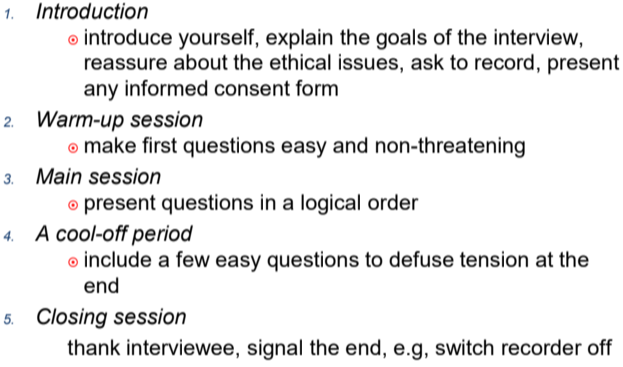
\includegraphics[scale=0.5]{assets/intervista.png}
	\end{center}

	Le linee guida per una corretta esecuzione di un'intervista sono:
	\begin{itemize}
		\item creare un clima amichevole e informale
		\item non dare opinioni personali
		\item non anticipare le risposte
		\item non guidare gli utenti nelle risposte
		\item non presentare una serie di opzioni tra cui scegliere
		\item porre domande semplici e chiare
		\item formulare una domanda per volta
		\item assicurarsi che l'utente abbia compreso la domanda
		\item concedere all'utente il tempo necessario per rispondere
		\item se non si ottiene la risposta desiderata, riprovare parafrasando la domanda, senza mai condurre l'utente alla risposta da dareadattare le domande alle risposte precedenti, senza seguire rigorosamente il piano preparato per l'intervista
		\item evitare l'utilizzo di termini tecnici o ambigui
		\item raccogliere esempi
		\item mostrarsi spontanei, semplici e flessibili, lasciando che l'utente fornisca informazioni in un qualsiasi ordine
		\item ascoltare l'utente, anche quando si dilunga in altri discorsi, e cercare di riportarlo sull'argomento senza evidenziare l'accaduto
	\end{itemize}

	Una volta eseguita l'intervista, si procede con l'analisi dei dati raccolti strutturando gli stessi in tabelle (una per utente) con osservazioni e fatti principali ricavati da registrazioni e appunti. Successivamente si raggruppano le tabelle in base alle analogie nei dati dei vari utenti ed etichettare le categorie risultanti. Infine, si effettua un resoconto finale per ogni categoria deducendo solo ciò che si può dimostrare.
	\vspace{\baselineskip}\\
	Questi risultati possono essere utilizzati nelle varie fasi di design e implementazione in modo da accertarsi che si stia procedendo secondo i bisogni dell'utente individuati tramite l'intervista. Inoltre possono usare aspetti evidenziati come spunto per l'ideazione e lo sviluppo di nuove caratteristiche dell'applicazione oppure come mezzo di risoluzione dei problemi evidenziati dall'utente durante l'intervista.\\
	Nello specifico si possono utilizzare le interviste durante le fasi di:
	\begin{itemize}
		\item \textbf{Analisi dei requisiti}: per individuare i bisogni e le aspettative degli utenti e definire i requisiti del sistema.
		\item \textbf{Progetto}: per valutare le specifiche dei requisiti, le funzionalità del sistema e le soluzioni di design.
		\item \textbf{Implementazione}: per individuare i problemi evidenti durante l'utilizzo del sistema e valutare le modifiche necessarie.
		\item \textbf{Valutazione}: per valutare l'usabilità e l'esperienza d'uso del sistema e identificare i problemi di usabilità.
	\end{itemize}

	\subsection{Focus Group}
	Il focus group è una tecnica di raccolta dati che coinvolge un gruppo di utenti in una discussione strutturata per raccogliere informazioni qualitative sui loro bisogni, aspettative e comportamenti sotto vari punti di vista. I focus group sono utilizzati per esplorare le opinioni e le percezioni degli utenti su un determinato argomento, per identificare i problemi e le sfide che affrontano e per generare idee e soluzioni innovative.
	I componenti di un focus group sono:
	\begin{itemize}
		\item Guidatore: guida la discussione, pone domande e stimola la conversazione.
		\item Osservatore: osserva e registra la discussione, prende appunti e raccoglie informazioni.
		\item Partecipanti: utenti che partecipano alla discussione, condividono le loro opinioni e le loro esperienze.
	\end{itemize}
	E' importante osservare direttamente il dialogo dei partecipanti e partecipare attivamente alla discussione in modo da mettere in relazione gli obiettivi degli utenti con i compiti e le azioni, capire come gli utenti scelgono i compiti per raggiungere i loro obiettivi, individuare i fattori ambientali e organizzativi che influenzano il loro lavoro e in che modo, e capire come gli utenti valutano il successo dei loro compiti.
	\vspace{\baselineskip}\\
	Questa tecnica è ispirata dall'etnografia, ovvero la disciplina che si basa sull'osservazione diretta e la partecipazione attiva per comprendere le culture e le società umane, e può essere utilizzata per studiare i comportamenti e le pratiche degli utenti in un contesto specifico.

	\subsection{Osservazione sul campo}
	L'osservazione sul campo è una tecnica di raccolta dati che coinvolge l'osservazione diretta degli utenti durante l'utilizzo del prodotto per identificare problemi di usabilità e migliorare l'esperienza dell'utente. L'osservazione sul campo può essere condotta in vari contesti, come l'ambiente di lavoro dell'utente, la sua casa o il luogo in cui svolge le sue attività quotidiane. Per effettuare un'osservazione sul campo, è necessario:
	\begin{itemize}
		\item \textbf{Definire l'obiettivo dell'osservazione}: Identificare gli obiettivi dell'osservazione e le informazioni che si vogliono raccogliere.
		\item \textbf{Selezionare il contesto}: Identificare il contesto in cui si svolgerà l'osservazione e pianificare le attività da osservare.
		\item \textbf{Individuare i partecipanti e le sedi}: Identificare i partecipanti all'osservazione e le sedi in cui si svolgerà.
		\item \textbf{Programmare le visite}: Pianificare le visite sul campo e definire il tempo e la durata dell'osservazione.
		\item \textbf{Selezionare gli utenti da osservare}: Identificare gli utenti da osservare e ottenere il loro consenso per partecipare all'osservazione.
		\item \textbf{Condurre l'osservazione}: Osservare direttamente gli utenti durante l'utilizzo del prodotto e prendere appunti sui problemi di usabilità e le aree di miglioramento.
		\item \textbf{Raccogliere i dati}: Raccogliere i dati raccolti durante l'osservazione e organizzarli in modo da poterli analizzare e interpretare. Si potranno utilizzare media come videoregistratori, audioregistarori, fotocamere, carta e penna, moduli prestampati, ecc.
	\end{itemize}

	\subsection{Scenari d'uso}
	Durante la progettazione e lo sviluppo di un prodotto potremmo tendere a concentrarci sull'oggetto della progettazione trascurando il contesto d'uso; tendiamo a vedere noi stessi come utenti tipici errando il punto di vista dell'utente o sottovalutiamo l'importanza di quest'ultimo rischiando di mancare la correttezza del prodotto.
	\vspace{\baselineskip}\\
	Per evitare questi errori, è possibile utilizzare gli scenari d'uso, ovvero storie immaginarie ma tipiche di uso del sistema da parte di persone fittizie ma concrete, che rappresentano bisogni, contesti e modalità d'uso tipiche del sistema da progettare. In questo modo otteniamo contesto, concretezza e visione oggettiva mettendo in evidenza requisiti inespressi.
	\vspace{\baselineskip}\\
	Gli scenari d'uso devono mettere in scena situazioni d'uso tipiche ma non ovvie, non devono contenere dettagli irrilevanti allo scopo, eevono essere complete (indicando le motivazioni e le conseguenze dell'uso del prodotto nella particolare situazione) e possono essere realizzati con tecniche diverse.
	\paragraph{Esempio di scenario d'uso}
	Progettazione di un sistema di prenotazione via web per un albergo di prima categoria di Catania
	\begin{itemize}
		\item \textbf{Persona}: Luigi, ingegnere di 35 anni, sposato, lavora in una società edile. Viaggia spesso per lavoro o vacanza, in Italia e all'estero, e si tratta bene. Non è mai stato in Sicilia
		\item \textbf{Scenario d'uso}: Luigi deve andare a Catania per lavoro. Desidera prenotare una camera in un albergo di prima categoria vicino alla filiale della sua azienda, che si trova in centro ad un passo da Piazza del Duomo. Deve pagare con American Express intestata all'azienda per politica aziendale. Starà a Catania due notti, forse tre. Preferisce alberghi moderni e desidera una camera doppia per uso singolo.
	\end{itemize}
	Lo scenario contiene molti requisiti impliciti:
	\begin{itemize}
		\item visualizzare sulla mappa di Catania gli alberghi di prima categoria
		\item mostrare la mappa in modo che Piazza del Duomo sia facilmente individuabile
		\item mostrare delle fotografie dell'albergo
		\item permettere di prenotare camere doppie a uso singolo
		\item accettare pagamenti con carta American Express
		\item non addebitare subito l'intero immporto del soggiorno per via della durata variabile.
	\end{itemize}

	\subsection{Questionari}
	I questionari sono uno strumento di raccolta dati che coinvolge la somministrazione di un elenco di domande strutturate a un campione di utenti per raccogliere informazioni quantitative sui loro bisogni, aspettative e comportamenti. I questionari possono essere utilizzati per raccogliere informazioni su larga scala, per confrontare le opinioni di un gran numero di utenti e per identificare tendenze e pattern nei dati raccolti. Sono meno flessiibili delle interviste poichè le domande sono predefinite e non possono essere modificate durante la somministrazione avendo minori possibilità di approfondimento. 
	\vspace{\baselineskip}\\
	Le domande non devono essere ambigue, devono essere chiare e semplici, il questionario deve essere breve. Nel caso contrario, si consiglia di adottare degli incentivi per la compilazione. Possono contenere domande aperte o chiuse. Sono sempre preferibili domande chiuse poichè più facili da analizzare e da somministrare.
	\vspace{\baselineskip}\\
	Dopo la somministrazione del qustionario, le risposte vengono convertite in dati e analizzate per identificare tendenze e pattern nei dati raccolti.
	\vspace{\baselineskip}\\
	Ci sono vari tipi di domande a risposta chiusa:
	\begin{itemize}
		\item \textbf{Domande a scelta multipla}: l'utente deve scegliere una o più risposte tra diverse opzioni.
		\item \textbf{Scalari}: l'utente deve giudicare un'asserzione specifica in base ad una scala numerica.
		\item \textbf{Checklist}: semplici risposte alternative, in numero limitato.
		\item \textbf{Rating Scale}: 
		\begin{itemize}
			\item \textbf{Likert Scale}: l'utente deve esprimere il proprio grado di accordo o disaccordo con un'affermazione su una scala a 5 o 7 punti.
			\item \textbf{Semantic Differential Scale}: l'utente deve esprimere il proprio giudizio su un concetto o un oggetto utilizzando coppie di aggettivi da incrociare.
		\end{itemize}
	\end{itemize}
	
	\subsection{Confronto di tecniche di raccolta dati}
	Le tecniche di raccolta dati presentano diversi utilizzi, vantaggi e svantaggi a seconda del metodo scelto. I questionari sono utili per rispondere a domande specifiche e permettono di raggiungere molte persone con poco sforzo. Tuttavia, devono essere progettati con grande accuratezza, altrimenti le risposte potrebbero risultare poco informative, e il tasso di risposta può essere basso.

	Le interviste individuali sono impiegate per esplorare diversi aspetti di un problema e i punti di vista correlati. Offrono il vantaggio di permettere all'intervistatore di guidare la conversazione verso i temi più rilevanti, ma richiedono molto tempo e possono non ottenere risposte schiette su argomenti delicati.

	I focus group si concentrano su argomenti specifici, coinvolgendo più persone e punti di vista. Tra i vantaggi c'è la possibilità di far emergere il consenso e soluzioni condivise. D'altro canto, la loro gestione richiede esperienza e c'è il rischio che alcune persone monopolizzino la discussione.

	Le osservazioni sul campo aiutano a comprendere il contesto in cui l'utente opera. Questo metodo fornisce una conoscenza diretta dell'uso reale di un prodotto, ma può risultare complesso da eseguire e richiede notevoli risorse in termini di tempo e impegno.

	I suggerimenti spontanei degli utenti permettono di identificare bisogni specifici o miglioramenti per un prodotto. Questo approccio è caratterizzato da bassi costi di raccolta, ma tende a produrre dati limitati e sporadici.

	Infine, l'analisi della concorrenza e delle best practices è utile per individuare le soluzioni migliori adottate in un determinato settore. Tale approccio consente di evitare di ripetere errori già noti e di ottenere un vantaggio competitivo, ma comporta costi elevati e l'impiego significativo di tempo e risorse.

	\section{Caso d'uso}
	Un caso d'uso è un insieme di interazioni finalizzate ad uno scopo utile per l'utente, fra l'utente (o più utenti) e il sistema. Ha un nome e una descrizione che ne definisce lo scopo, solitamente verbo + complemento oggetto.\\
	Un caso d'uso può essere composto da un insieme di task, ciascuno dei quali sarà a sua volta composto da un insieme di azioni elementari. Ovviamente si parla delle azioni che compie l'utente, non di ciò che fa il sistema.\\
	Un task è un insieme strutturato delle attività richieste, usate e ritenute necessarie per raggiungere un obiettivo. Spesso incluse sottotasks, ovvero attività che possono essere scomposte in attività più piccole.\\
	Task e azioni possono cambiare in base alle persone che li svolgono.

	\subsection{Analisi dei task}
	L'analisi dei task è utile per comprendere la natura del lavoro e identificare quali sono i task rilevanti considerando il coinvolgimento degli utenti, la loro analisi per capire come essi eseguono le varie attività nel'ambiente di lavoro. E' simile alla tecnica degli scenari, dalla quale sono stati eliminati il contesto ed altri dettagli.

	\subsubsection{Tipi e Livelli}
	Ci sono vari tipi di analisi dei task:
	\begin{itemize}
		\item \textbf{Workflow Analysis}: analisi dei processi di lavoro per identificare i task e le attività coinvolte quando sono coinvolte  più persone.
		\item \textbf{Job Analysis}: analisi dei processi di lavoro di un singolo individuo nell'arco di una giornata, settimana o mese lavorativo.
		\item \textbf{Task List}: analisi dei task che sono eseguiti da tutte le persone che potrebbero essere coinvolte nell'uso del sistema.
		\item \textbf{Task Sequence}: analisi dell'ordine di esecuzione dei task.
		\item \textbf{Procedure Analysis}: analisi delle procedure e delle scelte che sono seguite per eseguire un task o parte di esso.
		\item \textbf{Task Hierarchy}: analisi della struttura gerarchica dei task per comprendere come suddividere un task complesso in task più piccoli.
	\end{itemize}

	\subsection{Scenario vs Caso}
	Sono due cose diverse con obiettivi differenti.\\
	Gli scenari d'uso sono storie tipiche molto concrete di uso del sistema, raccontate con particolari per comprendere le motivazioni e il contesto e fare emergere eventuali requisiti impliciti.\\
	I casi d'uso fanno riferimanto a ruoli astratti dei vari attori e contiene solo informazioni sull'interazione che questi hanno con il sistema, senza alcuna informazione aggiuntiva sul contesto.
	
	
	\chapter{UCD Sprint}
	L'UCD Sprint è un approccio iterativo e incrementale alla progettazione e allo sviluppo di prodotti e servizi che coinvolge gli utenti fin dall'inizio del processo di sviluppo. L'UCD Sprint si basa su un ciclo di sviluppo iterativo che prevede la realizzazione di prototipi, la valutazione con gli utenti e il miglioramento continuo del prodotto. Questo approccio consente di identificare i problemi di usabilità e migliorare l'esperienza dell'utente in modo rapido ed efficace. Si basa sul modello cenerale dello HCD (ISO 9241-210).
	\begin{center}
		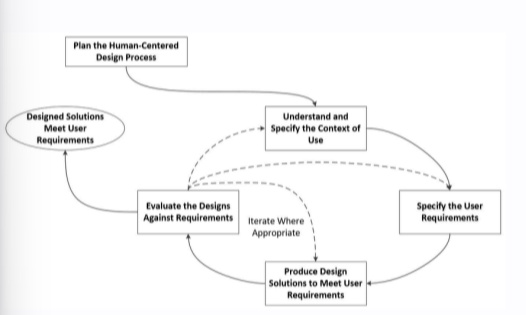
\includegraphics[scale=0.5]{assets/ucd.png}
	\end{center}
	Nello specifico, ad ogni iterazione il modello suggerisce attività specifiche da fare utilizzando metodi di HCI per identificare i requisiti degli utenti, sviluppare prototipi che implementano soluzioni di progetto, valutare gli stessi prototipi e, a seconda della valutazione, ripetere il ciclo o passare alla fase di sviluppo.
	\vspace{\baselineskip}\\
	Possiamo dividere il processo iterativo in 3 macroaree: discovery, design e reality check.
	\begin{center}
		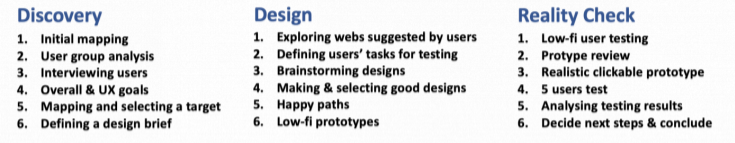
\includegraphics[scale=0.5]{assets/ucd2.png}
	\end{center}

	\section{Discovery}
	La fase di discovery è la prima fase del processo di sviluppo e si concentra sulla comprensione delle esigenze e dei bisogni degli utenti. Durante questa fase, vengono condotte attività di ricerca per identificare i gruppi di utenti che potrebbero utilizzare il prodotto, i loro bisogni e le loro aspettative. Le attività di ricerca possono includere interviste, focus group, osservazioni sul campo e analisi documentale. L'obiettivo della fase di discovery è identificare i requisiti degli utenti e definire le specifiche del prodotto. il risultato di questa prima fase di discovery sarà un'initial map che riassume i bisogni e le aspettative degli utenti e fornisce una visione generale del prodotto.
	\begin{center}
		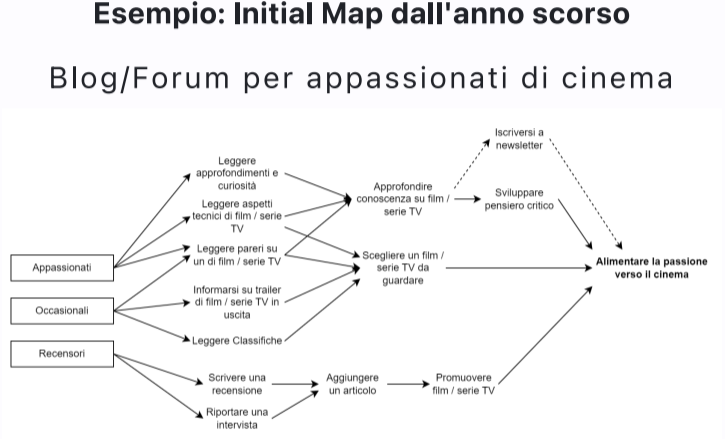
\includegraphics[scale=0.5]{assets/discovery.png}
	\end{center}
	Successivamente si andrà ad analizzare ogni gruppo di utenti elencati nell'initial mapping, anaizzando tutti i fattori riportati nel modello. Questo ci permetterà di ricavare un outcome mapping.
	\begin{center}
		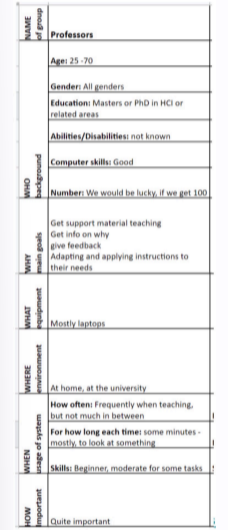
\includegraphics[scale=0.5]{assets/outcome.png}
	\end{center}
	Una volta ottenuto l'outcome mapping, si procederà con la raccolta dei requisiti tramite interviste o altri metodi di raccolta dati. Questi requisiti saranno utilizzati per definire le specifiche del prodotto. 
\end{document}